%%%%%%%%%%%%%%%%%%%%%%%%%%%%%%%%%%%%%%%%%%%%%%%%%%%%%%%%%%%
% EPFL report package, main thesis file
% Goal: provide formatting for theses and project reports
% Author: Mathias Payer <mathias.payer@epfl.ch>
%
% This work may be distributed and/or modified under the
% conditions of the LaTeX Project Public License, either version 1.3
% of this license or (at your option) any later version.
% The latest version of this license is in
%   http://www.latex-project.org/lppl.txt
%
%%%%%%%%%%%%%%%%%%%%%%%%%%%%%%%%%%%%%%%%%%%%%%%%%%%%%%%%%%%
\documentclass[a4paper,11pt,oneside]{report}
% Options: MScThesis, BScThesis, MScProject, BScProject
\usepackage[MScThesis,lablogo]{EPFLreport}
\usepackage{xspace}
\usepackage{listings}
% Enable all todo comments.
\usepackage[]{todonotes}
% Uncomment this to disable the comment blocks
% \usepackage[disable]{todonotes} 
% This is how we do comments for papers in the lab. This way you can see it 
% both in TeX and when you compile the PDF. Make sure they're all removed for 
% the final version by switching the lines above. I also don't mind if you 
% delete them once resolved because I can see them changed in git :)
\newcommand{\ant}[1]{\todo[inline,color=blue!40]{Antony: #1}}
\newcommand{\dam}[1]{\todo[inline,color=red!40]{Damian: #1}}
\newcommand{\lou}[1]{\todo[inline,color=green!40]{Louis: #1}}

\lstset{ 
  basicstyle=\footnotesize,
  frame=single,
  language=C++,
}

\title{Recovering type information from compiled binaries\\to aid in 
instrumentation}
\author{Louis Merlin}
\supervisor{Antony Vennard}
\adviser{Prof. Dr. sc. ETH Mathias Payer}
%\coadviser{Second Adviser}
\expert{Damian Pfammatter}

\newcommand{\sysname}{FooSystem\xspace}

\setlength{\parindent}{0cm}

\begin{document}
\maketitle
\makededication
\makeacks

\begin{abstract}
% The abstract serves as an executive summary of your project.
% Your abstract should cover at least the following topics, 1-2 sentences for
% each: what area you are in, the problem you focus on, why existing work is
% insufficient, what the high-level intuition of your work is, maybe a neat
% design or implementation decision, and key results of your evaluation.

The analysis of closed-source C++ programs is an arduous task.
C++ adds several powerful functionalities to the C language, which leads to
complex binaries.

Knowledge of class types and hierarchies can prove valuable during the reverse
engineering process.
Fortunately, some of that information can be recovered from stripped binaries
due to the way polymorphism is implemented in C++ compilers.
\lou{TODO : try striping binaries with more complex tools}

With the dis-cover tool, we are able to extract class information and the
hierarchy tree from a stripped C++ binary, and write DWARF debug information
and symbols for the later use of that knowledge by any existing debugging tool.
Through this method, we aim to demonstrate an open and collaborative way of
writing static analysis tools.

Through careful research of the way C++ exceptions are implemented, we are also
able to augment the capabilities of the RetroWrite static rewriting tool to
support C++ binaries.
We also show how the class information extracted by dis-cover could be used to
improve the instrumentation done by RetroWrite

By utilizing these two tools, we are able to successfully reverse engineer
several well-known large projects.
\lou{reverse engineer is not the right word => rewrite maybe ? Instruments ?}
\lou{We will give a cool example here if we end up with one.}

\end{abstract}

% \begin{frenchabstract}
% For a doctoral thesis, you have to provide a French translation of the
% English abstract. For other projects this is optional.
% \end{frenchabstract}

\maketoc

%%%%%%%%%%%%%%%%%%%%%%
\chapter{Introduction}
%%%%%%%%%%%%%%%%%%%%%%

% The introduction is a longer writeup that gently eases the reader into your
% thesis~\cite{dinesh20oakland}. Use the first paragraph to discuss the setting.
% In the second paragraph you can introduce the main challenge that you see.
% The third paragraph lists why related work is insufficient.
% The fourth and fifth paragraphs discuss your approach and why it is needed.
% The sixth paragraph will introduce your thesis statement. Think how you can
% distill the essence of your thesis into a single sentence.
% The seventh paragraph will highlight some of your results
% The eights paragraph discusses your core contribution.

% This section is usually 3-5 pages.


% Setting: compiled binaries; RetroWrite; [need for a compatible exchange 
% format => DWARF;] closed-source C++ binaries in the wild (android?).

Work on C++ began in 1979, as a "C with classes"~\cite{cwithclasses}.
Since then, the language has grown in popularity, and even surpassed C 
itself~\cite{stackoverflowpopularity}.
Examples of well-known C++ projects include modern browsers like 
Chrome~\cite{chrome} and Firefox~\cite{firefox}, the Qt Framework~\cite{qt}, or 
the zoom~\cite{zoom} conferencing software.
Nevertheless, reverse-engineering efforts have been focused towards C binaries, 
because analysis methods found this way will often work on C++ binaries too.


% Main challenge:
% C++-specific ELF sections are not as well documented as they could be (?);
% Debuggers do not work as well as they should on non-C binaries;

This has meant reverse engineering tools like Ghidra~\cite{ghidra}, IDA 
Pro~\cite{ida} or Binary Ninja~\cite{binja} have treated non-C binaries as 
second-class citizen.
These tools will often show C++ specific features as passing comments, failing 
to show the real implications of a try/catch block or a polymorphic class.

% Ghidra/IDA will show as pseudo-C code, but not C++
%  see throw/catch or RTTI
% C++ is quite a compilicated language.
% C's abstractions work very well in assembler, but C++ adds a whole layer of 
% complexity.
% When translated to assembly, a lot of information is lost.

The blame can mostly be put on the complexity of C++ when compared to C.
Whereas C translates quite naturally to assembly, abstractions specific to C++ 
require more work and complexity to be translated to asm.
This also leads to important information being lost from C++ source code to 
binary, but also certain information remaining.


% Related work:
% RetroWrite only does C;
% debugging tools don't have nice support for C++ features;
% DWARF will be explored more and more in the coming years;

The recent RetroWrite~\cite{dinesh20oakland} project by the HexHive lab is a 
static rewriting tool for x86\_64 position-independent binaries.
It enables the instrumentation of projects when we do not have access to the 
source code.
This can include a legacy project, a closed-source product or even malware.

% Does anything else try to do retrowriting C++ ?
% Does anything else try to extract classes ? (Marx / plugins)


% Our approach:
% Tool for static analysis of C++ binaries, to recover classes and display them 
% in a helpful way;
% Fixing RetroWrite to support C++ binaries;

In this thesis we would like to present the 
\textbf{dis-cover}~\cite{discovergithub} static analysis tool,
as well as improvements made to RetroWrite to support C++ binaries.


% Why it is needed:
% Non-obtrusive way of adding C++ support in debugging tools;
% Nobody (?) (as far as we know / to the best of our knowledge) has been able 
% to rewrite C++ binaries before, this could lead to very interesting 
% discoveries;

The dis-cover tool is able to extract information from a C++ binary, and 
re-inject it as debug information using the DWARF format into the binary.
This enables other debugging tools to see and display this information.


% Highlight results:
% 53\% of packages on Debian that use C++ have extracteable classes;
% [whatever we are able to do with C++ and RetroWrite];


% It's a first symbolic representation of C++ code that can be recompiled


% Core contribution:
% dis-cover as an open-source tool;
% [whatever we are able to add to RetroWrite];
% Also the documentation of the process.

[IF WE SUCCEEDED]
In this thesis we would like to show how we brought C++ support to RetroWrite, 
and what research opportunities this will create.

[IF WE FAILED]
In this thesis we will detail how we tried to bring C++ support to RetroWrite, 
and what remains to be done for the implementation to work.


%%%%%%%%%%%%%%%%%%%%
\chapter{Background}
%%%%%%%%%%%%%%%%%%%%

% The background section introduces the necessary background to understand your
% work. This is not necessarily related work but technologies and dependencies
% that must be resolved to understand your design and implementation.

% This section is usually 3-5 pages.

\section{Executable and Linkable Format (ELF)}

The common standard \textbf{Executable and Linkable Format} (ELF) format is 
mostly used as executable files, object code and shared libraries.
It usually contains a program header table, which describes memory segments 
(e.g. "this is read-only data", "this is executable instructions").
It also usually contains a section header table, describing sections (their 
name, size, offset and some flags). 
The rest of an ELF file is taken up by sections.
Famous sections include
\textbf{.text} (where the instructions are),
\textbf{.data} (where you will see global tables and other variables),
\textbf{.rodata} (you will find strings in here)
and \textbf{.eh\_frame} (where exception unwinding information is stored for 
C++ binaries).

\section{Position-Independent Code (PIC) and Executable (PIE)}
\label{picpie}

Position-independence for code is a property that guarantees that code will 
execute correctly no matter the absolute address of the body of code.
This is made possible by computing \textbf{relative positions} instead of
using absolute addresses, as well as a feature called \textbf{relocations}.

PIC is most often found for shared libraries, so that they can be inserted into 
an ELF file without worry.
PIE binaries are seen as more secure because they allow for easy inserting of 
security measures like address space layout 
randomization~\cite{aslr}.
We will talk more about PIE in \autoref{retrowritesection}.

\section{C++ features}

\subsection{Polymorphism}
\label{polymorphism}

% C++ polymorphism (what, how, but also research like Marx) (+ exceptions) 
% also talk about how compilers will optimize this out in certain situtations
The C++ programming language implements polymorphism.
This feature enables complex code logic that can comply with external business 
logic.
Here we will introduce the example that will follow us throughout this thesis :
in \autoref{classes} we define two abstract base classes \textbf{Animal} and 
\textbf{Feline},
and the two classes \textbf{Cat} (that inherits from Animal and Feline) and 
\textbf{Dog} (that inherits from Animal).
In a large code base, with multiple teams of programmers working on different 
features,
an Animal could be passed around without caring about whether it was a Cat, a 
Dog or any other species.
This Animal is sure to overwrite the \textbf{speak} method have whatever other 
properties and methods Animal has defined.
This logic is verified by the compiler.

\begin{figure}[h]
\begin{lstlisting}
class Animal {
public:
  virtual void speak() = 0
};

class Feline {
  virtual void retract_claws() {}
};

class Cat : public Animal, public Feline {
public:
  virtual void speak() { cout << "Purr" << endl; }
};

class Dog : public Animal {
public:
  virtual void speak() { cout << "Woof" << endl; }
};
\end{lstlisting}
\caption{Polymorphic classes in C++}
\label{classes}

\end{figure}

This polymorphism feature also enables re-use of functionality by inheriting 
parent classes.
If you want to implement a Lemur and your Animal class already has an 
implementation of the eat method,
you don't need a lemur-specific implementation if appropriate. 

Polymorphic classes are defined by having at least one virtual method, which is 
inheritable and overridable.
With this polymorphism comes type conversion, of which there are two kinds.
The first, \textbf{static\_cast}~\cite{staticcast}, will check that the
conversion is upcasting at compile time,
but does not do any run-time checks to verify the validity of the conversion.
An example of upcasting is converting a pointer of a \textbf{Cat} to a pointer
of an \textbf{Animal}.
The fact that a class is polymorphic will have no impact on this type of 
casting.
The second is the more interesting one for us. It is the 
\textbf{dynamic\_cast}~\cite{dynamiccast} expression.
Dynamic casting is a safe kind of type conversion that can handle downcasting 
and sidecasting.
An example of downcasting is converting a pointer of an \textbf{Animal} to a
pointer of a \textbf{Cat}. This is not guaranteed to work.
An example of sidecasting is converting a pointer of an \textbf{Animal} to a
pointer of a \textbf{Feline}. This is also not guaranteed to work (if the
Animal pointer was that of a Dog for example).
In order to achieve a dynamic cast, the system must have some kind of
information about the object's data type at run time.

This is where Run-Time Type Information (\textbf{RTTI}) comes into the picture.
The system will use this RTTI to infer type inheritance for dynamic casting.
We will now go into implementation details of RTTIs and virtual tables
(\textbf{VTables}), which point to them.

To make VTables and RTTIs appear in your C++ binary, you will to define
classes that inherit from each other, as well as at least one virtual method
in one of these classes.
\autoref{classes} shows an example of such classes.
You will also need to instantiate these classes, and have some logic to make
the class logic run-time dependent. 
This is extremely common in practice, as it is the core motivation for
polymorphism in the first place.
For an example, see the conditional dynamic cast between the two child classes
we defined in \autoref{classes}.
If you do not do these things, the class logic is likely to be abstracted away
by the compiler for optimization reasons.

\begin{figure}[h]

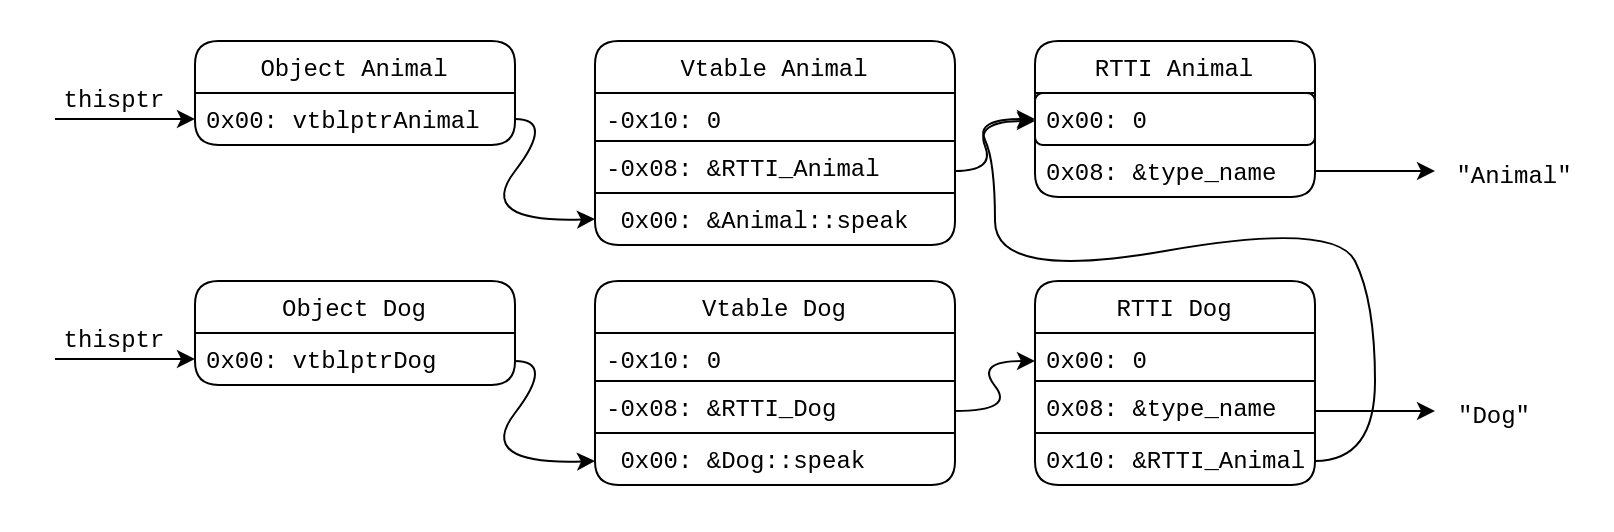
\includegraphics[width=16cm]{RTTI_graph.png}
\caption{Overview of an example of VTables and RTTI in memory}
\label{rttigraph}

\end{figure}

The structure of VTables and RTTIs is detailed in \autoref{rttigraph}.
All of this is defined in the Itanium C++ ABI~\cite{cppabi}.
An instance of a virtual class Animal will contain the \textbf{vtblptrAnimal}, 
a pointer to the virtual table (\textbf{VTable}) for the Animal class.
This VTable will be shared by all instances of this class (even by instances
of a class that inherits from Animal), and will contain pointers to the virtual
methods of the class.
The first value preceding the VTable is a pointer to the RTTI of the class. A
program finds out the class inheritance of a class instance at runtime by
following this pointer.

The RTTI itself is composed of a pointer to a VTable for the typeinfo class 
(defined by the compiler) and well as a pointer to the type name (this type 
name is not removed by simple stripping of the binary, like with 
\textbf{objdcopy --strip-all}).
This name is mangled using C++ mangling, and can trivially be demangled.
Here are some examples of C++ name mangling :
\textbf{\_ZTI6Feline} demangles to \textbf{typeinfo for Feline};
\textbf{\_ZTV6Feline} demangles to \textbf{vtable for Feline}.
Mangling is especially useful when defining several methods in the same scope 
with different arguments (this is called overloading), in order to
differentiate the different methods.
Mangling is also useful because of special characters in class names, like the
\textbf{::} characters who separate namespaces.
The next values of the RTTI are pointers to the RTTIs of the parent classes.
These are used at runtime to check the relationship between classes.
See \autoref{rttigraph} for an example, with the Dog RTTI containing a pointer 
to the Animal RTTI.


\subsection{Exceptions}
\label{exceptions}

Exceptions are one of the defining features that make C++ stand out from C.
In contrast to C errors, which terminate the whole program, C++ exceptions
can be caught and handled.

In order for the program to be able to continue execution after an exception
is caught, binaries need some way of safely doing \textbf{stack unwinding}.
The information on how to safely unwind the stack is stored in the
\textbf{.eh\_frame} section. It is encoded in a format similar to DWARF data
(see \autoref{dwarf}).

\subsection{Global constructors and frame dummy}
\label{framedummy}

During the execution of an ELF file, some methods will be run before the main
program starts. Pointers to these methods are stored in the
\textbf{init\_array}.
A simple C++ binary that uses exceptions will have an initialization array
containing a pointer to the \textbf{frame\_dummy}. This method is in charge of
setting up the stack frames to be able to unwind the frame during exception
handling later on.
In the initialization array, you will also find pointers to a global
constructor for every compilation unit (usually, a compilation unit is a C++
source file).

\section{DWARF debugging standard}
\label{dwarf}

\ant{MOAR!! :) There is quite a bit you can say here. DWARF powers debuggers, 
and lets you do things like map source to binary code, recover variable 
names, function names that might not be external symbols, as well as class 
information.
Another key point to mention for later will be the structure of how it is used 
in EH\_Frame. DWARF uses an abstract representation of the processor, so its 
register 1 for example must be mapped to the processor.}
\lou{Regarding Antony's comment => more info about the justification for using 
DWARF.}
% DWARF DIEs
\textbf{DWARF} is the debugging standard used widely in conjunction with 
executable ELF files.
It is often included in these ELF files in the \textbf{.debug\_info} section 
(and other related sections).
This debug information is made up of Debugging Information Entries 
(\textbf{DIEs}).
These entries can contain information about variable names, method definitions, 
the compilation process, or more importantly for us, class names and class 
inheritance. You can also map source code to binary code.
All of this information is usually used in debuggers.

The \textbf{.eh\_frame} section mentioned in \autoref{exceptions} is also used
by debuggers to unwind the stack for debugging purposes.

DWARF data takes the form of a tree of values.
The root of the tree is called the \textbf{Compile Unit} (CU).
It contains information about the source code file, the programming language
used as well as the compiler.

\section{RetroWrite} \label{retrowritesection}

% How RetroWrite works

The \textbf{RetroWrite}\cite{dinesh20oakland} project is a project from the
HexHive lab that aims to statically rewrite binaries and instrument them, to
improve fuzzing capabilities.
Static binary rewriting is the process of taking a binary file, and modifying
it such that there is a patch applied to it but the other functionalities
remain the same.

RetroWrite's core idea is to symbolize all of the addresses in the machine
code. This means transforming an an address offset (+8) into a symbol
(.LD1234) and adding the appropriate label at that location.
These labels will be used by the assembler to compute the addresses of
functions and data offsets for example.
This way, we can add any instruction after and before existing instructions
without breaking relative offsets.

RetroWrite only works on \textbf{x86\_64} position-independent executables
(see \autoref{picpie}), compiled from C. This enables the RetroWrite to stay
heuristics-free (meaning that it is designed to work for every example without
exceptions).


%%%%%%%%%%%%%%%%
\chapter{Design}
%%%%%%%%%%%%%%%%

% Introduce and discuss the design decisions that you made during this project.
% Highlight why individual decisions are important and/or necessary. Discuss
% how the design fits together.

% This section is usually 5-10 pages.

\section{Goals}

The primary goal of this project was to extract some debug information from a
stripped C++ binary, make it available through DWARF in order to be able to
use that information in other projects, as a proof of concept.
The hope is that this process will be re-used in other projects in the future.
For this project, we decided to focus on recovering class information from
Run-Time Type Information (RTTI, see \autoref{polymorphism}).

% Design => Decisions
% We decided not to reproduce Marx's work
% First attempt : recover classes from RTTI
% Future work : could take approaches like Marx and re-feed it like us
Class recovery from compiled C++ binaries has been tried multiple ways before:
there are plugins for popular debugging tools, like 
ida\_gcc\_rtti~\cite{idagccrtti} for IDA Pro (which requires a license),
or Ghidra-Cpp-Class-Analyzer~\cite{ghidracppclassanalyzer} for Ghidra
(but this information is only usable inside of the Ghidra debugger);
there are academic projects such as MARX~\cite{marx} that rely on heuristics 
around VTables to find classes and inheritance information.
The MARX project can recover classes when no RTTI is present (in the Chrome 
project for example, where the \textbf{-fno-rrti} compilation flag is used),
with around 90\% accuracy.

\subsection{Finding Run-Time Type Information}

% VTable => RTTI
%   mention class data (Debian analysis)
As we mentioned in the Background chapter, the RTTIs are available for a
class hierarchy tree when there is at least one virtual method implemented
by one of the classes.
We decided to test if RTTIs occurred often in the wild : we proceed to download 
every Debian package that listed C++ as a dependency (get the list with 
\textbf{apt-cache rdepends libgcc1} on a Debian machine).
Out of around 80'000 packages, 5827 of them list C++ as a dependency.
Out of those, we extracted classes from 3194 (54\%).
This does not mean that the other 46\% of packages do not use classes,
because in many cases these classes are optimized away by the compiler
(in the more straightforward cases).
We will share more details about this experiment in the Evaluation chapter.
\lou{Add link to Evaluation chapter}

When looking at a binary's VTables and RTTIs, we only need to look for a
specific subset of them : the primary base virtual tables and their RTTIs.
There is one of each for each class defined in the binary. Secondary virtual
tables occur when there is multiple inheritance and complex method overwrites.
They define only a subset of a class' methods, and do not contain RTTIs.
We can differentiate the two kinds of virtual tables by the presence of an
offset at the beginning of the VTable : a primary base virtual table will have
a value of $0$ as an offset, whereas a secondary virtual table will have an
offset to the primary base virtual table.

\lou{This could be diagrammed (RTTIs) => multiple inheritance, diamond 
problem...}

\subsection{DWARF}
\label{dwarfdesign}

\lou{Alternatives to DWARF ? Maybe on MacOS and Windows ? Maybe I should say
debugging in **unix** binaries}

% Why do we want DWARF data ?
%   We want to make the info available to reversing tools
%   => input from Dr. Sergey Bratus
%        He would like to see DWARF used as a lingua franca for debugging
% Also, exception's try/catch blocks & exception types
% but dwarf is limited for this (=> future work)
Once we have extracted class information from RTTI, next comes the question :
what should we do with all of this class information ? What would be the most
useful format to output the data in ?
This is where DWARF~\cite{dwarf} comes in the picture. DWARF is the debugging 
standard for programs.
It is mostly used by developers trying to understand where their implementation 
fails,
and by reverse engineers to get a better understanding of how a program was 
conceived (although DWARF information is usually stripped from proprietary 
software).
This kind of debug data is mostly found in compiled binaries, written in C,
C++ or Rust for example. 
By having DWARF data as an output, the information would become readable by 
most modern reversing tools.

There is a current push for DWARF to become the lingua franca for reverse 
engineering tools, lead by researchers like Dr. Sergey Bratus~\cite{bratus} 
from DARPA.
He has published a paper in 2011 where he was able to exploit certain features 
of DWARF to control program execution : Exploiting the hard-working 
DWARF~\cite{hardworkingdwarf}.
In it, they prove that the DWARF information used during exception handling
is Turing-complete and can be used to embed exploits in executables.

DWARF data is structured as a tree of \textbf{Debug Information Entries} 
(DIEs). These entries contain a \textbf{tag} and a list of
\textbf{attributes}.
These entries can describe how the original code is written, as well as
information about classes, variables, types, and other structures in the
binary.

The DWARF format also uses abbreviations to compress the debug information.
Instead of re-describing a DIE every time, their structure is defined in an
abbreviation table (stored in the \textbf{debug\_abbrev} section of the ELF
file).
Each DIE will have an index in that table, which describes its tag and list
if attributes names and types. The rest of the DIE is the list of its
attributes, in the order they were defined in the abbreviation.

In this project, we use very minimalist DIE abbreviations, containing only
what we could infer from the analysis.

% Injecting debug section & symbols
With dis-cover, we are able to inject information in the debug and symbol 
sections of the binary, creating a new ELF file with all of this useful info 
included.
We will go more into the implementation details in \autoref{dwarfdump} and
\autoref{wrappingimplementation}. \lou{figure 4.1 ?}

\subsection{Exceptions}

% Also: exceptions (we felt this needed to be handled)
Exceptions are often implemented as classes, and dis-cover will naturally 
recover information about programmer-defined exceptions.
Future extensions of this work might consider recovering more information about 
exceptions.

% RetroWrite structure
%  x86_64 userspace and kernel, and arm_64
%  We've decided to focus on the x86_64 userspace
%    Most widely used target
%    Kernel drivers are mostly written in C
% We still want to keep the deterministic ability of retrowrite
We had to study and work with exceptions and exception handling frames for 
the augmentation of RetroWrite with C++ capabilities (see
\autoref{retrowriteimplementation}).
Today, RetroWrite supports the reversing of x86\_64 position-independent 
binaries.
There was also work to augment RetroWrite to support kernel 
code~\cite{rwkernel} and arm\_64~\cite{rwarm}.
We aimed to add C++ capabilities for x86\_64 binaries only, as it is the most 
widely used platform (though the same logic will most probably apply with a 
little tweaking to ARM and other architectures).
\lou{Kernel target is not one we are going to consider because C++ is not used
to its full extend}

\section{RetroWrite}
\label{retrowritedesign}

The first bug we encountered while trying to use RetroWrite on C++ binaries
was due to the fact that the \textbf{initialization array} (see
\autoref{framedummy}) contained a pointer to the \textbf{frame dummy} and this
was not handled well during RetroWrite's symbolization process.
By adding special treatment for that scenario, we were able to resolve this
failure.

Once that was fixed, we saw that using RetroWrite on binaries that had C++
exception handling would cause crashes in the new binary, caused by the fact
that the exceptions thrown were never caught.
Exception behavior is described in the \textbf{Language Specific Data Area}
(LSDA), which is found in the \textbf{.gcc\_except\_table} section of the ELF
file.
This LSDA describes, row by row, actions to take for specific instruction in
the code we are hitting while dealing with a thrown exception. These actions
could be : destructing an out-of-scope variable, or examining a catch clause
to see if they should catch the current exception.

\section{Design for future integrations}

As described in \autoref{dwarfdesign}, we use the DWARF format as an output
for the extracted information. This makes the knowledge easily reusable in
other reverse engineering projects.

For example, dis-cover output could be used in RetroWrite in order to add
instrumentation around \textbf{Object Type Integrity}, as defined in the CFIXX
paper~\cite{cfixx}, or reinforcing type checks as defined in the HexType
paper~\cite{hextype} to avoid type confusion errors and vulnerabilities.

We also were able to design dis-cover in a heuristics-free way, which fits
perfectly with RetroWrite's current goal to avoid heuristics.


%%%%%%%%%%%%%%%%%%%%%%%%
\chapter{Implementation}
%%%%%%%%%%%%%%%%%%%%%%%%

% The implementation covers some of the implementation details of your project.
% This is not intended to be a low level description of every line of code that
% you wrote but covers the implementation aspects of the projects.

% This section is usually 3-5 pages.

% Python script (because RetroWrite; and good tools) (1 sentence)
We decided to write a python module for this project, as the python ecosystem 
has great reverse engineering packages, and for easy integration in RetroWrite, 
which is also written in python.

\section{Finding RTTIs}

% RTTI and VTable
The first thing dis-cover does is find ELF sections where the VTables and RTTIs 
could be hiding.
This is usually \textbf{.rodata} (read-only data) and \textbf{.data.rel.ro}, 
but could sometimes also be related sections like \textbf{.data.rel.ro.local}, 
or \textbf{.rdata}.
As per the Itanium C++ ABI, the base VTable of a class will contain an 
"offset-to-top", which will be 0 in the primary base virtual table's case, 
followed by a pointer to an RTTI.
\lou{Actually these are pointers -2 and -1 (-0x10 and -0x08)}
We simply have to pattern-match for zeroes directly followed by a pointer to 
another part of the read-only data sections, and we have a potential RTTI 
pointer.

\lou{Add link to figure, it's easier to understand to an image / or a similar
figure that helps better understand **this** part}

Next, we analyze the data at the pointer's value.
We check that we have not already extracted a class at that address, and if
not, we assert the following address is a pointer to a string located in a
read-only data section.
If it is, we can extract that string, demangle it, and we have a class name,
a virtual table address and an RTTI address that we have extracted.
The next values in the RTTI are pointers to the RTTIs the class inherits from.
We can go through them and parse them if we have not already, to add this 
inheritance information to the extracted class.

This algorithm is $O(n)$, as adding a class only adds one more value to parse.

\section{Creating DWARF data}

% Creating DIEs
Next, we want to add that information to the debug sections of a new ELF file.

% DIE Bytecode
In order to write DWARF data, the first step is defining the types we will be 
using, and their fields.
This is done by writing bytes in the \textbf{.debug\_abbrev} section.
For example, we create an abbrev of type \textbf{class\_type}, which has a 
\textbf{name}, and can have sub-field (children).
Then, we create the abbrev of type \textbf{inheritance}, which has a 
\textbf{type} (a reference to the parent type).

We can then populate the \textbf{.debug\_info} with classes and their 
inheritance data.
DWARF data takes the form of a tree of values. We have to create a 
\textbf{compile\_unit} value at the root, and then the branches will be 
\textbf{class\_type}s.
These \textbf{class\_type}s will themselves have as children 
\textbf{inheritance} values if the class inherits from another class.
\autoref{dwarfdump} shows a very simple example of this, with two class types 
and one inheriting from the other.

\begin{figure}[h]
\begin{lstlisting}
< 1><0x0000001a>    DW_TAG_class_type
                      DW_AT_containing_type       <0x0000001a>
                      DW_AT_calling_convention    DW_CC_pass_by_reference
                      DW_AT_name                  Shape
                      DW_AT_byte_size             0x00000008
< 1><0x00000026>    DW_TAG_class_type
                      DW_AT_containing_type       <0x00000026>
                      DW_AT_calling_convention    DW_CC_pass_by_reference
                      DW_AT_name                  Rectangle
                      DW_AT_byte_size             0x00000008
< 2><0x00000031>      DW_TAG_inheritance
                        DW_AT_type                  <0x0000001a>
\end{lstlisting}
\caption{Extract of a dwarfdump output showing simple inheritance}
\label{dwarfdump}
\end{figure}

The strings themselves are stored in another section, \textbf{.debug\_str}, and 
are referred to with their offset in that section.

\lou{The three dwarf sections should be explained in more detail in the 
Design section.}

\section{Creating symbols}

% symbols
Symbols are mainly used for shared object loading, to use the \textbf{printf}
method from \textbf{stdio.h} for example, the binary must be aware of a
method named \textbf{printf}. The same is true for
\textbf{system\_clock} in C++ for example.
Symbols are also used to have access to variable names, class names, function
names or any other kind of text information when debugging a binary.
In dis-cover, we want to create two symbols for every class we have found
during the analysis : one pointing to the VTable and one pointing to the RTTI,
and labeling them as such.

In order to create new symbol sections, we take the symbol table from the 
original binary (if there was one) and append the aforementioned symbols.

The two symbol sections are \textbf{.symtab}, which contains the information 
(offset, size, type, ...) for each symbol, and \textbf{.strtab}, which contains 
the strings related to these symbols.

\section{Wrapping things together}
\label{wrappingimplementation}

\subsection{Creating a fake ELF file}

% eu-unstrip etc
Once we have the three debug sections ready
(\textbf{.debug\_abbrev} with the debug types, \textbf{.debug\_info} with the 
debug information, and \textbf{debug\_str} with the strings)
as well as the two symbol sections, we have to make them available to the user.
They contain all of the information we were able to extract from the binary.
The first step is building an empty ELF file with only these five sections in 
them. We will discuss why in \autoref{combiningelf}.

We start by constructing a \textbf{program header table}.
This table contains information about the offset and size of each segment of 
the binary (which segment is used for what, and their read/write permissions).
The ELF file we're creating will not be run, but only used temporarily.
Thus, we noticed that we did not have to create a valid program header table 
for the process to work.
We simply copy this program header table almost as-is from the original binary.

Next, we use the individual sections we built earlier and construct the 
\textbf{section header table}.
For every section present in the original binary, we create an entry in the 
section header table, reusing most values from the original section header 
table.
The only values we modify is the offset.
For every section that we have created, we add the appropriate row in the 
section header table.
Every section name gets added to the \textbf{.shstrtab} section, as per the 
convention.

Finally, we construct the \textbf{elf header}, taking some of the values from 
the original binaries, and calculating some others from the size of the tables 
and sections we have built.
We can now create a fake ELF file by appending the elf header, the program 
header table, the sections we built and the section header table.

\subsection{Stripping the original ELF file}

Next, we will create a stripped version of the original ELF file.
We use the \textbf{objcopy --strip-all} command.
This is to avoid section conflicts in the next step.

\subsection{Combining the two ELF files}
\label{combiningelf}

Now, we can use the ELF utility program \textbf{eu-unstrip} to combine the two 
ELF files we have created into one.
The newly created combined ELF file will contain all of the code and data from 
the original file, as well as the debug and symbol sections we have created.

The reason why we had to go through these hoops to make the debug and symbol
information available to the user is because these sections do not come alone
: they have to be accompanied by machine code and data.
We did not want to recreate a whole compiler to assemble all of this data.
Luckily, the \textbf{eu-unstrip} tool was created as an utility application
to "combine stripped files with separate symbols and debug information".
In order to use this tool, we had to make the fake binary match the original
binary as closely as possible regarding headers and segments.

% what it does and does not do

\section{C++ capabilities in RetroWrite}
\label{retrowriteimplementation}
% RetroWrite implementation details
% Refer to the other thesis
% unwind tables etc

The first modification we did to RetroWrite to add support for C++ binaries
was to address the \textbf{init\_array} errors described in
\autoref{retrowritedesign}.
This meant treating the \textbf{frame\_dummy} method differently, as it was
ignored by the symbolizer.

The next modification was a larger one : the whole \textbf{Language Specific
Data Area} (LSDA) had to be symbolized and rewritten.
See \autoref{retrowritedesign} for more details.
This table, contained in the \textbf{.gcc\_except\_table} section, has offsets
to cleanup functions, as well as lengths of instructions (which we transform
into label differences).

The LSDA structure is quite complex, but in practice only a subset of actions
are used by C++ compilers to describe the logic of exception handling.

%%%%%%%%%%%%%%%%%%%%
\chapter{Evaluation}
%%%%%%%%%%%%%%%%%%%%

% In the evaluation you convince the reader that your design works as intended.
% Describe the evaluation setup, the designed experiments, and how the
% experiments showcase the individual points you want to prove.

% This section is usually 5-10 pages.

\section{Small case studies}

% Small examples
In addition to the first version of dis-cover, we created three small programs 
highlighting different features of C++.
One was using simple inheritance,
one had a namespace (which we can and should recover as part of the analysis),
and the last one was a use case of multiple inheritance (using the diamond 
problem).

We also created a script that would compile these three programs using
different levels of compiler optimization.
We could then use dis-cover to see if we could recover every class and the 
correct tree from the binaries.
This served as a useful benchmark to check whether dis-cover was functioning 
correctly if we tried to apply changes to it.

These examples alone were not capable of letting us evaluate the full 
capabilities of dis-cover.
We found a few big applications that could serve that purpose.

\section{Real-world case studies}

% Big applications examples
The first and smallest of these case studies was the \textbf{gold 
linker}~\cite{gold}.
We were able to find 571 classes in version 1.16 of the program.
This provides a good benchmark, but the classes themselves do not make use of 
multiple inheritance (only a "simple" inheritance tree).

\textbf{LibreOffice}~\cite{libreoffice} on the other hand provided us with a 
great test case :
the program is fragmented into many small libraries, containing some 
interesting uses of multiple inheritance.
See \autoref{libloglo} for an example of multiple inheritance in the 
\textbf{libloglo.so} library from LibreOffice.
This particular example was very important for verifying a big bug that was 
present in an early version of dis-cover.
After fixing the bug, we were noticing around 10\% more inheritance links in 
some projects (but not more classes).
Being able to go check with the open-source LibreOffice code that we had found 
the right inheritance links was extremely helpful.

\begin{figure}[h]

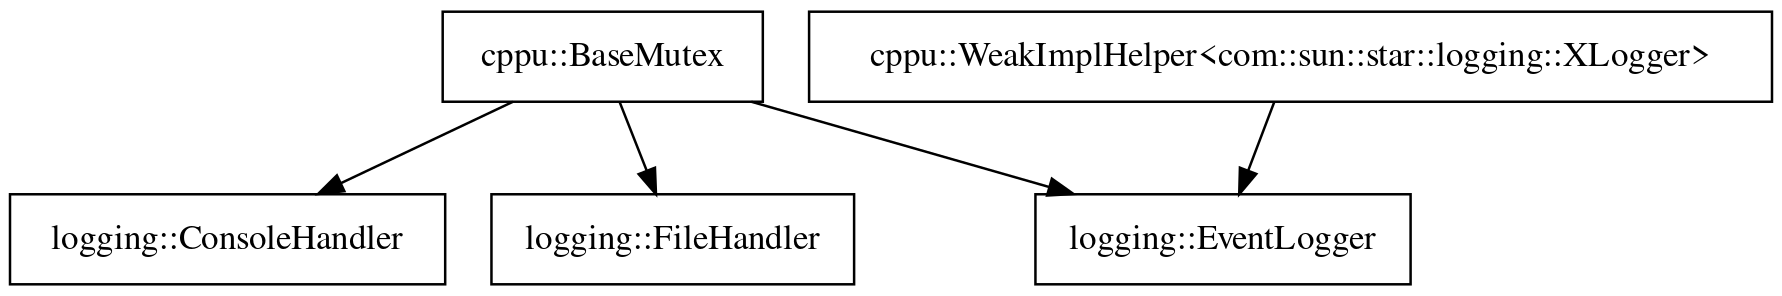
\includegraphics[width=16cm]{libloglo_partial.png}
\caption{Partial class tree of libloglo.so from LibreOffice}
\label{libloglo}

\end{figure}

Finally, we also were able to study the closed-source \textbf{zoom}~\cite{zoom} 
binary.
This test case is very interesting in two ways.
First, we are able to find \textbf{6039 classes} in the binary, with 
\textbf{5601 edges} in the class hierarchy graph.
Second, as a large (76M) and complex ELF file, it served as a perfect benchmark 
for the performance of the algorithm.
By adding a simple check earlier in the RTTI-spotting pipeline, we were able to 
speed up the analysis of the zoom binary 13.37 times, from over an hour to five 
minutes.

\autoref{discoverbenchmarks} details the benchmarks we conducted on many 
well-known projects.

\begin{table}[h]
  \centering
  {\small
  \begin{tabular}{l | r | r | r | r }
    ELF File and version & Size & Size of .rodata & Computation time & Amount 
of classes recovered  \\
    \hline
    gold 1.16 & 2.3M & 0.1M & 0m0.605s & 571 \\
    ceph-dencoder 15.2.13 & 29M & 0.9M & 0m12.493s & 2959 \\
    zoom 5.5.7938.0228 & 76M & 16M & 5m50.626s & 6039 
  \end{tabular}
  }

\caption{Benchmarks of dis-cover on a machine running Ubuntu 20.04 with a 2.6 
GHz dedicated vCPU}
\label{discoverbenchmarks}

\end{table}

% Debian test
As we have shown before, out of the 5827 Debian packages that list C++ as a 
dependency, we were able to extract classes from 3194 (54\%).
The total number of classes we found is 960'188, with 39\% of them unique 
across all packages (unique name in unique tree).

% RetroWrite test
\section{Testing RetroWrite}


%%%%%%%%%%%%%%%%%%%%%%
\chapter{Related Work}
%%%%%%%%%%%%%%%%%%%%%%

% The related work section covers closely related work. Here you can highlight
% the related work, how it solved the problem, and why it solved a different
% problem. Do not play down the importance of related work, all of these
% systems have been published and evaluated! Say what is different and how
% you overcome some of the weaknesses of related work by discussing the 
% trade-offs. Stay positive!

% This section is usually 3-5 pages.

\section{MARX}

MARX~\cite{marx} is a static analysis tool which is related to what dis-cover
is trying to achieve. Using analysis of the virtual tables in a C++ binaries,
they are able to accurately extract 90\% of the classes. This is done without
the need for RTTIs, and thus can target a larger number of projects (such as
the chrome browser and the Node.js runtime) at the cost of having a
probabilistic approach.

They use six heuristics to locate the virtual tables, related to the table
layout and content.

This project could be a great candidate for future integration into
RetroWrite, if we extend the tool to add defenses around type integrity for
example.

\section{Plugins}

There exists multiple plugins for reverse engineering frameworks that serve
the same purpose as dis-cover. For IDA Pro, there exists \textbf{IDA GCC RTTI}
~\cite{idagccrtti}, and for Ghidra there is the \textbf{Class and Run Time
Type Information Analyzer}~\cite{ghidracppclassanalyzer}.

These are very useful, and integrate very well into the reverse engineering
frameworks, but they cannot make that information available to other tools.

The IDA Pro plugin does offer the option to create a \textbf{.dot} graph file
that can be used to create a visual representation of the hierarchy tree.
\lou{This is a potential upgrade to dis-cover, a script has already been
written}

\section{Type Integrity}

\subsection{CFIXX}

\textbf{CFIXX}~\cite{cfixx} introduces \textbf{Object Type Integrity}, which
is a dynamic (runtime) mechanism that keeps track of object types and prevents
adversaries from overwriting type information to hijack the control flow.
It is applied at compile time.

A future project could use the classes extracted with dis-cover and the
rewriting capabilities of RetroWrite to implement object type integrity on
closed-source binaries.

\subsection{HexType}

\textbf{HexType}~\cite{hextype} aims to remove \textbf{type confusion errors}
from programs, by adding explicit run-time checks during compilation.
This is done even for objects that are not polymorphic, so as to remove all
of the attack surface.

\section{Exploiting the hard-working DWARF}

\textbf{Exploiting the Hard-Working DWARF}~\cite{hardworkingdwarf}
demonstrated that it was possible to incorporate exploits in the
\textbf{.eh\_frame} and \textbf{.gcc\_except\_table} sections.
They showed that the exception handling mechanism was a Turing-complete
language, and they proved they could take control of the system when an
exception was thrown.

This paper rekindled a global interest in DWARF as an academic research topic,
which lead to projects like this one.

%%%%%%%%%%%%%%%%%%%%
\chapter{Conclusion}
%%%%%%%%%%%%%%%%%%%%

In the conclusion you repeat the main result and finalize the discussion of
your project. Mention the core results and why as well as how your system
advances the status quo.

\cleardoublepage
\phantomsection
\addcontentsline{toc}{chapter}{Bibliography}
\printbibliography

% Appendices are optional
% \appendix
% %%%%%%%%%%%%%%%%%%%%%%%%%%%%%%%%%%%%%%
% \chapter{How to make a transmogrifier}
% %%%%%%%%%%%%%%%%%%%%%%%%%%%%%%%%%%%%%%
%
% In case you ever need an (optional) appendix.
%
% You need the following items:
% \begin{itemize}
% \item A box
% \item Crayons
% \item A self-aware 5-year old
% \end{itemize}

\end{document}
